% Author: Rasmus Pank Roulund
\documentclass{minimal}
\usepackage{tikz}
\usepackage{verbatim}

\begin{comment}
:Title: Credit rationing

An illustration inspired by a figure in Stiglitz, J.E. and Greenwald, B. (2003). `Towards a New Paradigm in Monetary Economics`__.

.. __: http://books.google.com/books?id=dZrI_dHoKgUC&dq=Towards+a+new+paradigm+for+monetary+economics&source=bn&ei=fDKXSbmrJMaC-gbQ_Pj8CA&sa=X&oi=book_result&resnum=4&ct=book-ref-page-link&cad=one-book-with-thumbnail

Parts of the source code are modified from https://sites.google.com/site/kochiuyu/Tikz

\end{comment}
\usetikzlibrary{arrows,calc}
\tikzset{
%Define standard arrow tip
>=stealth',
%Define style for different line styles
help lines/.style={dashed, thick},
axis/.style={<->},
important line/.style={thick},
connection/.style={thick, dotted},
}
\begin{document}


%%%%%%%%%%%%%%%%%%%%%%%%%%%%%%%%%%%%%%%%%%%%%%%%%%%%    
%%%%%%%%%%%%%%%%%%%%%%%%%%%%%%%%%%%%%%%%%%%%%%%%%%%%    
%%%%%%%%%%%%%%%%%%%%%%%%%%%%%%%%%%%%%%%%%%%%%%%%%%%%    



  \begin{tikzpicture}[scale=1]
    % Axis
    \coordinate (y) at (0,5);
    \coordinate (x) at (5,0);
    \draw[<->] (y) node[above] {$r$} -- (0,0) --  (x) node[right]
    {$\mathit{EV}$};
    % A grid can be useful when defining coordinates
    % \draw[step=1mm, gray, thin] (0,0) grid (5,5); 
    % \draw[step=5mm, black] (0,0) grid (5,5); 

    % Let us define some coordinates
    \path
    coordinate (start) at (0,4)
    coordinate (c1) at +(5,3)
    coordinate (c2) at +(5,1.75)
    coordinate (slut) at (2.7,.5)
    coordinate (top) at (4.2,2);

    \draw[important line] (start) .. controls (c1) and (c2) .. (slut);
    % Help coordinates for drawing the curve
    % \filldraw [black] 
    % (start) circle (2pt)
    % (c1) circle (2pt)
    % (c2) circle (2pt)
    % (slut) circle (2pt)
    \filldraw [black] 
     (top) circle (2pt) node[above right, black] {$Q$};

     % We start the second graph
     \begin{scope}[xshift=6cm]
       % Axis
      \coordinate (y2) at (0,5);
      \coordinate (x2) at (5,0);
      \draw[axis] (y2) node[above] {$r$} -- (0,0) --  (x2) node[right] {$L$};
      % Define some coodinates
     \path
     let
     \p1=(top)
     in
     coordinate (sstart) at (1,.5) 
     coordinate (sslut) at (4, 4.5)
     coordinate (dstart) at (4,.5)
     coordinate (dslut) at (1,4.5)
% Intersection 1
     coordinate (int) at  (intersection cs:
       first line={(sstart)--(sslut)},
       second line={(dstart)--(dslut)})
% Intersection 2
    coordinate (int2) at  (intersection cs:
       first line={(top)--($(10,\y1)$)},
       second line={(dstart)--(dslut)})
% Intersection 3
    coordinate (int3) at  (intersection cs:
       first line={(top)--($(10,\y1)$)},
       second line={(sstart)--(sslut)});
% Draw the lines
     \draw[important line] (sstart) -- (sslut) node[above right] {$S$}
       (dstart) -- (dslut)  node[above left] {$D$};
     \draw[connection] let \p1=(int2), \p2=(int3) in 
     (int2)--(\x1,0) node[below] {$\mathit{L_D}$}
     (int3)--(\x2,0) node[below] {$\mathit{L_S}$};
      \end{scope}
%Finally, connect the two graphs
     \draw[connection] let \p1=(top), \p2=(x2) in (0,\y1) node[left]
     {$r^*$} -- (\x2, \y1);
    \end{tikzpicture}
    
    
%%%%%%%%%%%%%%%%%%%%%%%%%%%%%%%%%%%%%%%%%%%%%%%%%%%%    
%%%%%%%%%%%%%%%%%%%%%%%%%%%%%%%%%%%%%%%%%%%%%%%%%%%%    
%%%%%%%%%%%%%%%%%%%%%%%%%%%%%%%%%%%%%%%%%%%%%%%%%%%%    

\newpage

%%% Long-run and short-run average cost curves
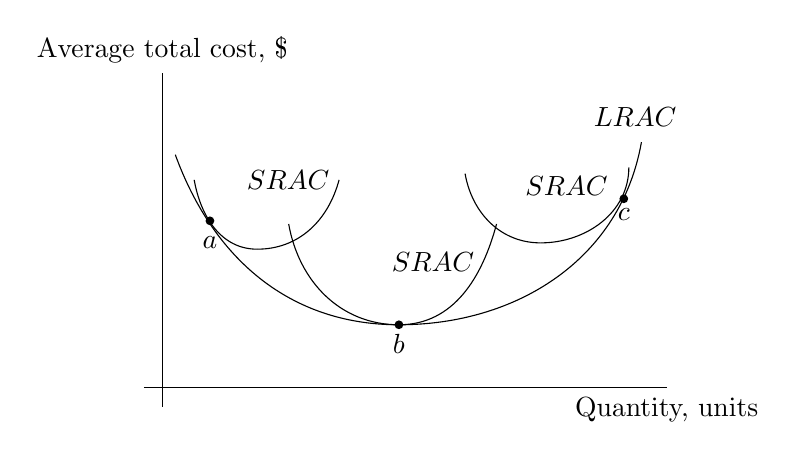
\begin{tikzpicture}[scale=0.8]
% Axis
\draw (-0.3,0)-- (0,0) -- (8,0) node [below] {Quantity, units};
\draw (0,-0.3)-- (0,0) -- (0,5) node [above] {Average total cost, \$};
%
\draw (0.2,3.7) to [out=290,in=180] (3.75,1);
\draw (3.75,1) to [out=360,in=260] (7.6,3.9);
\node [above] at (7.5,4) {$LRAC$};
%
\draw (0.5,3.3) to [out=280,in=180] (1.5,2.2);
\draw (1.5,2.2) to [out=360,in=255] (2.8,3.3);
\draw [fill] (0.75,2.65) circle [radius =0.06];
\node [below] at (0.75,2.55){$a$};
\node [left] at (2.8,3.3){$SRAC$};
%
\draw (2,2.6) to [out=280,in=180] (3.75,1);
\draw (3.75,1) to [out=360,in=255] (5.3,2.6);
\draw [fill] (3.75,1) circle [radius =0.06];
\node [below] at (3.75,1) {$b$};
\node [left] at (5.1,2) {$SRAC$};
%
\draw (4.8,3.4) to [out=280,in=180] (6,2.3);
\draw (6,2.3) to [out=360,in=270] (7.4,3.5);
\draw [fill] (7.32,3) circle [radius =0.06];
\node [below] at (7.32,3) {$c$};
\node [left] at (7.22,3.2) {$SRAC$};
%
\end{tikzpicture}


%%%%%%%%%%%%%%%%%%%%%%%%%%%%%%%%%%%%%%%%%%%%%%%%%%%%    
%%%%%%%%%%%%%%%%%%%%%%%%%%%%%%%%%%%%%%%%%%%%%%%%%%%%    
%%%%%%%%%%%%%%%%%%%%%%%%%%%%%%%%%%%%%%%%%%%%%%%%%%%%    

\newpage

% Production possibility frontier
\begin{tikzpicture}[scale=1.2]
% Axis
\draw (0,5.1) node [left] {$Y$} -- (0,0) node [below left] {$0$} -- (4,0) node [below] {$X$};
%
\draw (0,4.1) to [out=-15, in=120] (2.8,2) to [out=-60, in=95] (3.4,0);
% D --> E
\draw [->] (2.8,2) -- (3.3,2.2);
% A -- B
\draw [dashed] (1.2,3.6) -- (3.1,1.3);
% A -- C
\draw [dashed] (1.2,3.6) -- (2.9,3.2);
% Label "E"
\node [right] at (3.3,2.2) {$E$};
% Label "B"
\node [right] at (3.1,1.3) {$B$};
% Label "F"
\node [left] at (0,4.1) {$F$};
% Draw dot at F
\draw [fill] (0,4.1) circle [radius=.05];
% Label "H"
\node [right] at (0,4.5) {$H$};
% Draw dot at H
\draw [fill] (0,4.5) circle [radius=.05];
% Label "G"
\node [above left] at (3.4,0) {$G$};
% Draw dot at G
\draw [fill] (3.4,0) circle [radius=.05];
% Label "I"
\node [right] at (2.5,2.5) {$I$};
% Draw dot at I
\draw [fill] (2.5,2.5) circle [radius=.05];
% Label "D"
\node [above] at (2.9,2) {$D$};
% Draw dot at D
\draw [fill] (2.8,2) circle [radius=.05];
% Label "C"
\node [right] at (2.9,3.2) {$C$};
% Draw dot at ??
\draw [fill] (2.9,3.2) circle [radius=.05];
% Label at "A"
\node [above right] at (1.2,3.6) {$A$};
% Draw dot at A
\draw [fill] (1.2,3.6) circle [radius=.05];
\end{tikzpicture}


%%%%%%%%%%%%%%%%%%%%%%%%%%%%%%%%%%%%%%%%%%%%%%%%%%%%    
%%%%%%%%%%%%%%%%%%%%%%%%%%%%%%%%%%%%%%%%%%%%%%%%%%%%    
%%%%%%%%%%%%%%%%%%%%%%%%%%%%%%%%%%%%%%%%%%%%%%%%%%%%    

\newpage

% Template for aggregate demand and aggregate supply

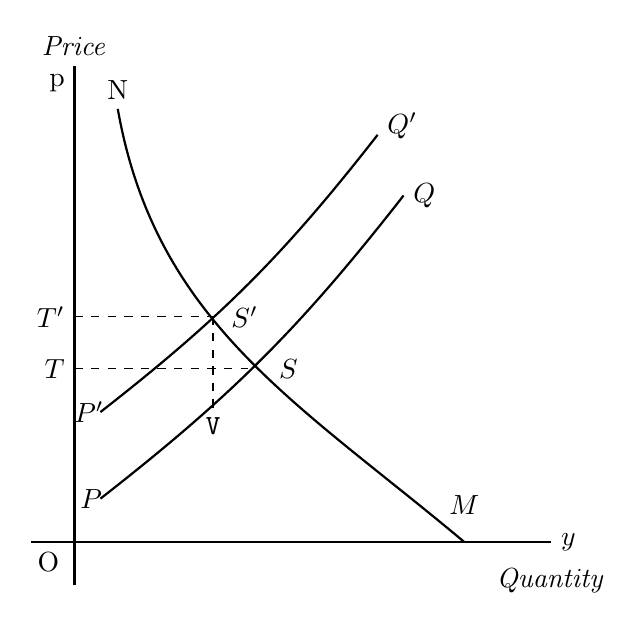
\begin{tikzpicture}[scale=1.1]
% Axis
\draw [thick] (-0.3,0) node [below] {O} (-0.5,0)-- (0,0) -- (5.5,0) node [right] {$y$};
\node [above] at (0,5.5) {\emph{Price}};
\node [below] at (5.5,-0.2) {\emph{Quantity}};
\draw [thick] (0,-0.5)-- (0,0) -- (0,5.5);
\node [left] at (0,5.3) {p};

%Downward slopping line
\node [above] at (0.5,5) {N};
\draw [thick] (0.5,5) to [out=280,in=140] (4.5,0);
\node [above] at (4.5,0.2) {$M$};

% Upward Slopping PQ
\draw [thick] (0.3,0.5) to [out=38,in=232] (3.8,4);
\node [left] at (0.43,0.5) {$P$};
\node [right] at (3.8,4) {$Q$};

% Upward Slopping P'Q'
\draw [thick] (0.3,1.5) to [out=38,in=232] (3.5,4.7);
\node [left] at (0.45,1.5) {$P'$};
\node [right] at (3.5,4.8) {$Q'$};

% dashed lines
\draw [dashed] (0,2.6)--(1.6,2.6);
\node [right] at (1.7,2.6) {$S'$};
\draw [dashed](1.6,1.55)--(1.6,2.6);
\node [below] at (1.6,1.55) {$\texttt{V}$};
\draw [dashed](0,2)--(2,2);
\node [right] at (2.25,2) {$S$};
\node [left] at (0,2) {$T$};
\node [left] at (0,2.6) {$T'$};


\end{tikzpicture}

    
    
    

%%%%%%%%%%%%%%%%%%%%%%%%%%%%%%%%%%%%%%%%%%%%%%%%%%%%    
%%%%%%%%%%%%%%%%%%%%%%%%%%%%%%%%%%%%%%%%%%%%%%%%%%%%    
%%%%%%%%%%%%%%%%%%%%%%%%%%%%%%%%%%%%%%%%%%%%%%%%%%%%    

\newpage


% The Marshallian measure of consumer surplus
\begin{tikzpicture}[scale=1]
% Axis
\draw [->] (0,0) node [below] {0} -- (0,0) -- (6,0) node [right] {$\emph{Quantity}$};
\draw [->] (0,0) node [below] {0} -- (0,0) -- (0,5.5) node [above] {$\emph{Price}$};
% Downward sloping curve
\draw (0,5)--(6,1.4);
% Label "D"
\node [right] at (6,1.4) {$D$};
% Segment P--A
\draw (0,3.5)--(2.5,3.5);
% Segment P'--B
\draw (0,2)--(5,2);
% Segment B-Q'
\draw (5,2)--(5,0);
% Segment Q--A
\draw (2.5,0)--(2.5,3.5);
% Label "B"
\node [right] at (5,2.2) {$B$};
% Label "A"
\node [right] at (2.5,4) {$A$};
% Label I
\node [right] at (.2,5.2) {$I$};
% Label P'
\node [left] at (0,1.5) {$P'$};
% Label P
\node [left] at (0,3.5) {$P$};
% Label Q
\node [below] at (2.2,0) {$Q$};
% Label Q'
\node [below] at (5,0) {$Q'$};
\end{tikzpicture}    
    
    
    
     
%%%%%%%%%%%%%%%%%%%%%%%%%%%%%%%%%%%%%%%%%%%%%%%%%%%%    
%%%%%%%%%%%%%%%%%%%%%%%%%%%%%%%%%%%%%%%%%%%%%%%%%%%%    
%%%%%%%%%%%%%%%%%%%%%%%%%%%%%%%%%%%%%%%%%%%%%%%%%%%%    

\newpage



\begin{tikzpicture}
\draw[thick,<->] (0,7) node[above]{$p$}--(0,0)--(8,0) node[right]{$q$};
\draw (0,6)--(6,0) node[above right]{D};
\draw (0,3) --(5,3) node[right]{$c_0$};
\draw(0,2) --(5,2) node[right]{$c_1$};
\draw[dashed] (0,4) node[left]{$p_1$}--(2,4)--(2,0) node[below]{$q_1$};
\draw[dashed] (0,3) node[left]{$p_0$}--(3,3)--(3,0) node[below]{$q_0$};
%\path[pattern=horizontal lines,pattern color=red] (2,4)--(2,3)--(3,3);
%\path[pattern=vertical lines,pattern color=blue] (0,3)--(2,3)--(2,2)--(0,2);
\end{tikzpicture}



%%%%%%%%%%%%%%%%%%%%%%%%%%%%%%%%%%%%%%%%%%%%%%%%%%%%    
%%%%%%%%%%%%%%%%%%%%%%%%%%%%%%%%%%%%%%%%%%%%%%%%%%%%    
%%%%%%%%%%%%%%%%%%%%%%%%%%%%%%%%%%%%%%%%%%%%%%%%%%%%    

\newpage



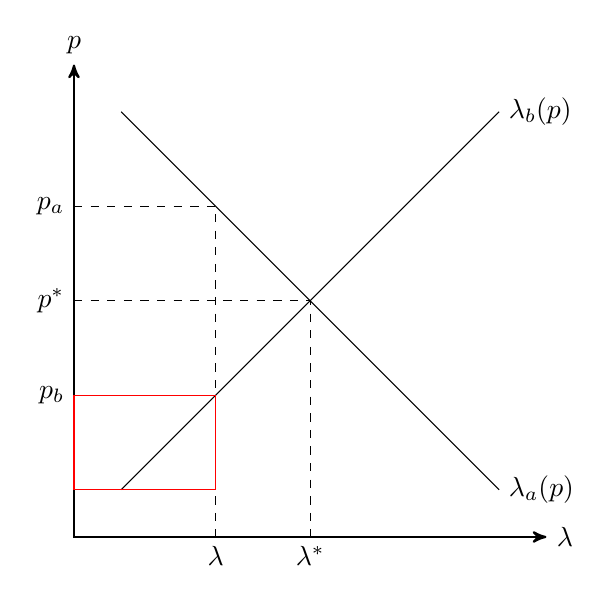
\begin{tikzpicture}[scale=0.6]
\draw[thick,<->] (0,10) node[above]{$p$}--(0,0)--(10,0) node[right]{$\lambda$};
\draw(1,1)--(9,9) node[right]{$\lambda_b(p)$};
\draw(1,9)--(9,1) node[right]{$\lambda_a(p)$};
\draw[dashed](0,5) node [left] {$p^*$}--(5,5)--(5,0) node [below] {$\lambda^*$};
\draw[dashed](0,7) node [left] {$p_a$}--(3,7)--(3,0) node [below] {$\lambda$};
\draw[dashed](0,3) node [left] {$p_b$}--(3,3);
%\draw[pattern=north west lines, pattern color=blue] (0,3) rectangle (3,7);
\draw[red] (0,3) rectangle (3,1);
\end{tikzpicture}



%%%%%%%%%%%%%%%%%%%%%%%%%%%%%%%%%%%%%%%%%%%%%%%%%%%%    
%%%%%%%%%%%%%%%%%%%%%%%%%%%%%%%%%%%%%%%%%%%%%%%%%%%%    
%%%%%%%%%%%%%%%%%%%%%%%%%%%%%%%%%%%%%%%%%%%%%%%%%%%%    

\newpage

\begin{tikzpicture}[scale=0.8]
\draw[thick] (0,9) node[above]{$P$}--(0,0) node[below right]{$0$}--(12,0) node[below]{$Y$};
\draw(1,1.5) ..controls (5,2) and (8,3) .. (8.5,9) node[above]{$AS$};
\draw (2,9) node[above]{$AD$}--(8.5,1.3);
\draw(8,9)--(8,0) node[below]{$Y_f$};
\draw[dashed](6.53,3.6)--(6.53,0) node[below] {$Y_e$};
\end{tikzpicture}


%%%%%%%%%%%%%%%%%%%%%%%%%%%%%%%%%%%%%%%%%%%%%%%%%%%%    
%%%%%%%%%%%%%%%%%%%%%%%%%%%%%%%%%%%%%%%%%%%%%%%%%%%%    
%%%%%%%%%%%%%%%%%%%%%%%%%%%%%%%%%%%%%%%%%%%%%%%%%%%%    

\newpage


% Keynesian cross diagram
\begin{tikzpicture}[scale=0.5]
%\scriptsize
\draw[thick] (0,12) node[above]{$E$}--(0,0) node[below right]{$0$}--(12,0) node[below]{$Y$};
\draw(0,2)--(12,11) node[right]{$C(Y)+I+G+X-M(Y)$};
\draw(0,0)--(12,12) node[right]{$E(Y)=Y$};
\draw[dashed](8,8)--(8,0) node[below]{$Y_e$};
\draw[dashed](10,9.5)--(10,0) node[below]{$Y_f$};
\draw (0,0) ++(0:2) arc(0:45:2);
\node [right] at (0.5,0.5) {45\textdegree};
\end{tikzpicture}


%%%%%%%%%%%%%%%%%%%%%%%%%%%%%%%%%%%%%%%%%%%%%%%%%%%%    
%%%%%%%%%%%%%%%%%%%%%%%%%%%%%%%%%%%%%%%%%%%%%%%%%%%%    
%%%%%%%%%%%%%%%%%%%%%%%%%%%%%%%%%%%%%%%%%%%%%%%%%%%%    

\newpage

% 
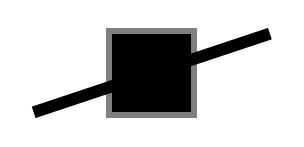
\begin{tikzpicture}[line width=1ex]
\draw (0,0) -- (3,1);
\filldraw [draw opacity=0.5] (1,0) rectangle (2,1);
\end{tikzpicture}


%%%%%%%%%%%%%%%%%%%%%%%%%%%%%%%%%%%%%%%%%%%%%%%%%%%%    
%%%%%%%%%%%%%%%%%%%%%%%%%%%%%%%%%%%%%%%%%%%%%%%%%%%%    
%%%%%%%%%%%%%%%%%%%%%%%%%%%%%%%%%%%%%%%%%%%%%%%%%%%%    

\newpage

% Price elasticity of demand

\begin{tikzpicture}[scale=3] 
% Draw axes
\draw [<->,thick] (0,2) node (yaxis) [above] {$P$}  |- (3,0) node (xaxis) [right] {$Q$};
% Draw two intersecting lines
\draw[ color=white ] (0,0) coordinate (a 1) -- (2 ,2) coordinate (a 2) ;
\draw (0 ,1.5) coordinate (b 1) -- (1.5 ,0) coordinate (b 2) node [ below ] {$Demand$};
% Calculate the intersection of the lines a 1 −− a 2 and b 1 −− b 2
% and store the coordinate in c.
\coordinate (c) at ( intersection of a 1--a 2 and b 1--b 2) ; 
% Draw a dot to indicate intersection point
\fill [red] (c) circle (1pt);
\draw[->,dashed] ($(c)+(0,0.15)$) -- ($(c)+(-.7,0.85)$);
\draw[->,dashed] ($(c)+(0.15,0)$) -- ($(c)+(.85,-0.7)$); 
\fill[blue] (0.5,1.5) node {Elastic};
\fill[blue] (1.6,0.5) node {Inelastic};
\draw[->] (1.5,1.5) node[label= above:Unitary Elastic] {} -- ($(c)+(.1,.1)$);
\end{tikzpicture}


%%%%%%%%%%%%%%%%%%%%%%%%%%%%%%%%%%%%%%%%%%%%%%%%%%%%    
%%%%%%%%%%%%%%%%%%%%%%%%%%%%%%%%%%%%%%%%%%%%%%%%%%%%    
%%%%%%%%%%%%%%%%%%%%%%%%%%%%%%%%%%%%%%%%%%%%%%%%%%%%    

\newpage



    
\end{document}
